%****************************************************************************%
%* KaDeploy Support                                                         *%
%*                                                                          *%
%* Author(s):                                                               *%
%* - Abdelkader AMAR (Abdelkader.Amar@ens-lyon.fr)                          *%
%* - David LOUREIRO (David.Loureiro@ens-lyon.fr)                            *%
%*                                                                          *%
%* $LICENSE$                                                                *%
%****************************************************************************%
%* $Id: GUM_Kadeploy.tex,v 1.3 2007/11/29 16:03:21 dloureir Exp $
%* $Log: GUM_Kadeploy.tex,v $
%* Revision 1.3  2007/11/29 16:03:21  dloureir
%* typo corrections
%*
%* Revision 1.2  2007/11/08 11:31:14  dloureir
%* Correcting the headers
%*
%****************************************************************************%
\chapter{Deploy your Kadeploy images}
KaDeploy is a fast and scalable deployment system for site and grid
computing. KaDeploy is the reconfiguration system used in \gfk, allowing
the users to deploy their own OS on their reserved nodes.

For more information about how to create and manage KaDeploy images, please
refer to the documentation available on the \gfk web page.

The Figure \ref{fig:GRUDU_kadeploy} shows the frame allowing you to deploy
images on which you have rights. The left hand side of the frame corresponds to
sites and nodes available for deployment (i.e. reserved with the deploy type).
 You can click on the checkboxes to select/deselect the nodes. If you want to 
select/deselect all nodes, you can click on the corresponding button on the 
right-hand side of the frame. Then you can select the image you want to deploy
from the lists on the right hand side of the frame.

When you are done with the configuration, you can click on the deploy
button. A new frame will be displayed corresponding to the log of the deployment
(with both standard output and error).

  \begin{figure}[H]
	\centering
	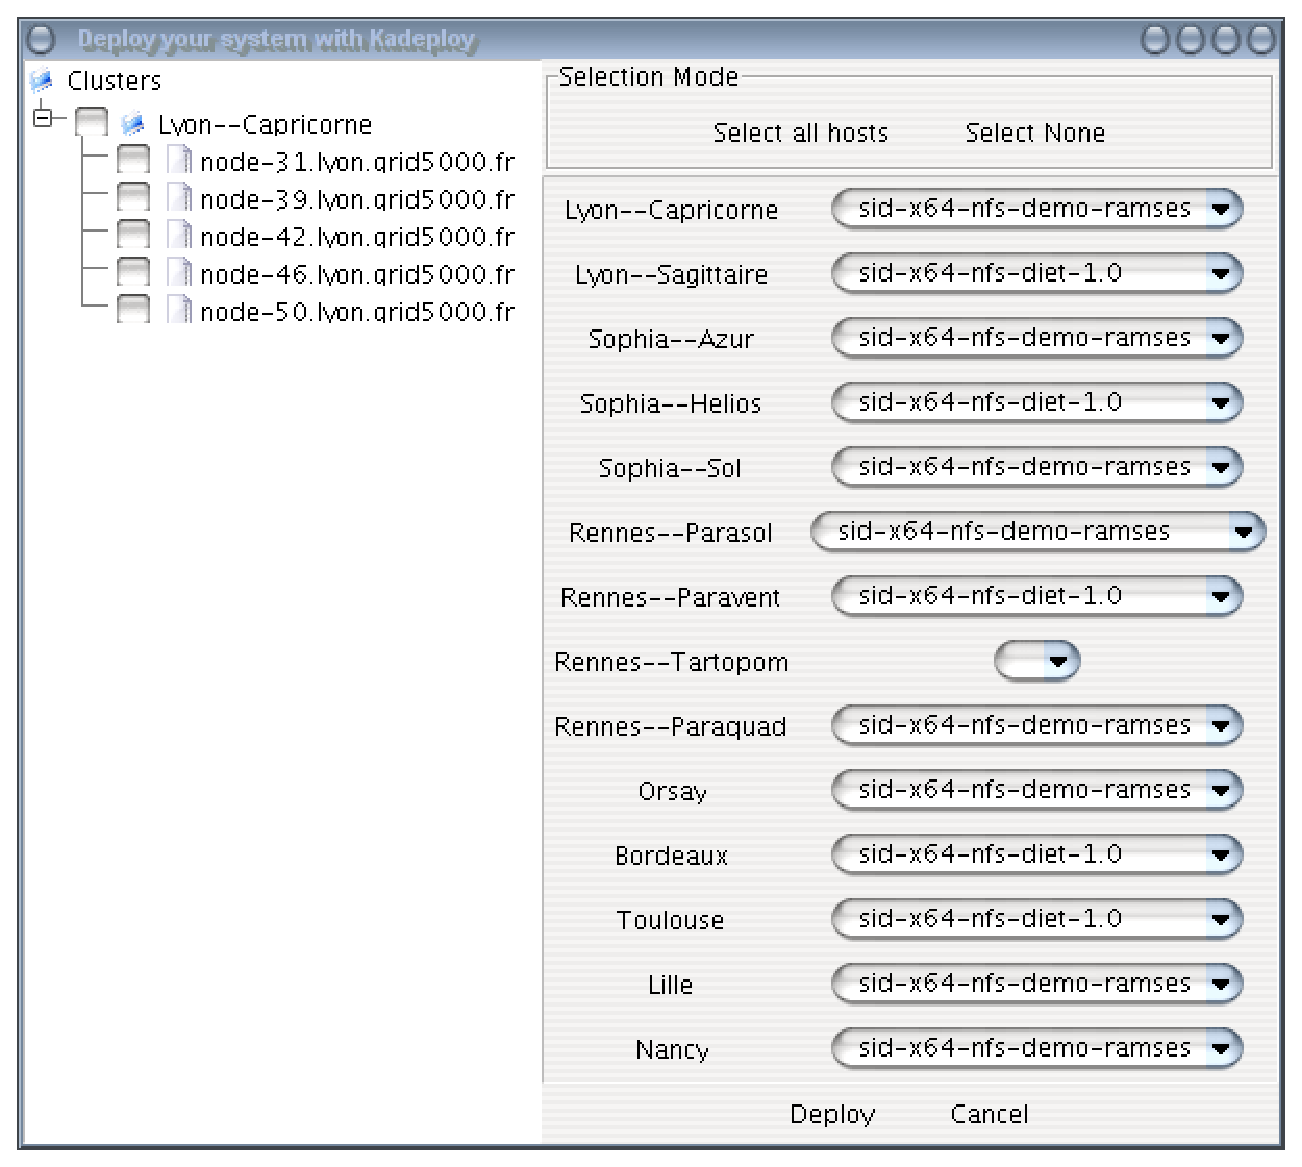
\includegraphics[width=0.5\linewidth]{figures/GRUDU_kadeploy.eps}
	\caption{Kadeploy frame}
	\label{fig:GRUDU_kadeploy}
  \end{figure}

%******************************************%